\section{IPMA}

\subsection{International Project Management Association}
\begin{frame}[allowframebreaks]{International Project Management Association}
	IPMA \foreign{International Project Management Association}
	\begin{itemize}
		\item Asociación Internacional dedicada al desarrollo y promoción de la \textbf{dirección de proyectos}.
		\item Organizada como una federación internacional de más de 55 asociaciones nacionales de dirección y gestión de proyectos.
	\end{itemize}
	
	\framebreak
	
	IPMA \foreign{International Project Management Association}
	
	\begin{itemize}
		\item Su actividad principal es la \textbf{certificación} de las competencias en dirección de proyectos.
		\item ICB \foreign{(IPMA Competence Baseline)}
		\begin{itemize}
				\item Marco desarrollado para las habilidades en dirección de proyectos, que sirve de base para el programa de certificación en \textbf{cuatro niveles}.
		\end{itemize}
		\item La certificación abarca competencias técnicas, contextuales y del comportamiento, y ha de renovarse cada cierto tiempo.
	\end{itemize}
	
	\framebreak
	
	Un poco de historia.
	
	\begin{itemize}
		\item El origen de la IPMA se remonta a 1964.
		\item Un grupo internacional de directores de proyectos se reune para discutir los beneficios del método.
		\item En 1965 este grupo de debate funda en Suiza una asociación, la actual IPMA, bajo el nombre de IMSA \foreign{(International Management Systems Association)}.
		\item El primer congreso internacional tuvo lugar en 1967 en Viena, con participantes de 30 países diferentes.
	\end{itemize}
	
	\framebreak
	
	Niveles de certificación que establece IPMA en dirección de proyectos:
	
	\begin{enumerate}
		\item \textbf{IPMA Nivel A} \emph{(Certified Projects Director)}
		\item \textbf{IPMA Nivel B} \emph{(Certified Senior Project Manager)}
		\item \textbf{IPMA Nivel C} \emph{(Certified Project Manager)}
		\item \textbf{IPMA Nivel D} \emph{(Certified Project Management Associate)}
	\end{enumerate}
	
	Cada una de ellas tiene una duración de 5 años.
	
	\framebreak
	
	\begin{block}{IPMA Nivel A \emph{(Certified Projects Director)}}
		\begin{itemize}
			\item \textbf{Competencias:} Será capaz de gestionar carteras o programas.
			\item \textbf{Requisitos:} Para obtenerlo se debe tener como mínimo cinco años de experiencia en dirección de carteras, dirección de programas o dirección de multiproyectos.
		\end{itemize}
	\end{block}
	
		\begin{block}{IPMA Nivel B \emph{(Certified Senior Project Manager)}}
			\begin{itemize}
				\item \textbf{Competencias:} Será capaz de dirigir proyectos complejos.
				\item \textbf{Requisitos:} Para obtenerlo se debe tener como mínimo cinco años de experiencia en dirección de proyectos.
			\end{itemize}
		\end{block}
	
	\framebreak
	
	\begin{block}{IPMA Nivel C \emph{(Certified Project Manager)}}
		\begin{itemize}
			\item \textbf{Competencias:} Será capaz de dirigir proyectos de complejidad limitada o de gestionar un subproyecto de un proyecto complejo en todos los elementos de competencia de la dirección de proyectos.
			\item \textbf{Requisitos:} Para obtenerlo se debe tener como mínimo tres años de experiencia en dirección de proyectos.
		\end{itemize}
	\end{block}
	
	\begin{block}{IPMA Nivel D \emph{(Certified Project Management Associate)}}
		\begin{itemize}
			\item \textbf{Competencias:} Tendrá conocimientos de dirección de proyectos en todos los elementos de competencia.
			\item \textbf{Requisitos:} No es obligatoria ninguna experiencia previa para obtenerlo.
		\end{itemize}
	\end{block}
	
	\framebreak
	
	Beneficios de los programas de certificación:
	
	\begin{itemize}
		\item \textbf{Para el personal de dirección de proyectos:} obtener un certificado con reconocimiento internacional que dé fe de su competencia en la dirección.
		\item \textbf{Para los proveedores de servicios de dirección de proyectos:} una demostración de la competencia profesional de sus empleados.
		\item \textbf{Para los clientes:} Mayor certeza de que recibirán los servicios más avanzados de un director de proyectos.
	\end{itemize}
\end{frame}

\subsection{AEIPRO (IPMA en España)}

\begin{frame}[allowframebreaks]{AEIPRO (IPMA en España)}
	AEIPRO \foreign{Asociación Española de Ingeniería de Proyectos}
	\begin{itemize}
		\item Asociación sin ánimo de lucro que tiene por objetivo el desarrollo del campo de la \textbf{Dirección e Ingeniería de Proyectos}.
		\item Nace en 1992 y desde el año 1999 es la asociación española representante de \textbf{IPMA} \foreign{(International Project Management Association)}.
	\end{itemize}
	
	\framebreak
	
	Para conseguir el proceso de certificación en España de IPMA(AEIPRO) se han de seguir los siguientes pasos:
	
	\begin{enumerate}
		\item El aspirante contactará con la secretaría indicando su interés por participar en alguna convocatoria e indicando el nivel.
		\item La secretaría pedirá al aspirante que envíe la solicitud de evaluación correspondiente al nivel solicitado.
		\item El aspirante justifica el abono de la tasa y firma la solicitud devolviéndola a la secretaría, así como los impresos de CV.
		\framebreak
		\item La secretaría devuelve aceptación o denegación una vez estudiada la documentación, y se notifica para la asistencia a la prueba.
		\item El candidato realiza la prueba.
		\item La secretaría informa de los resultados directamente al candidato.
		\item Se entrega el diploma acreditativo al ahora ya recién certificado y se actualizan los registros de certificados.
		
		\framebreak
		
		\begin{center}
			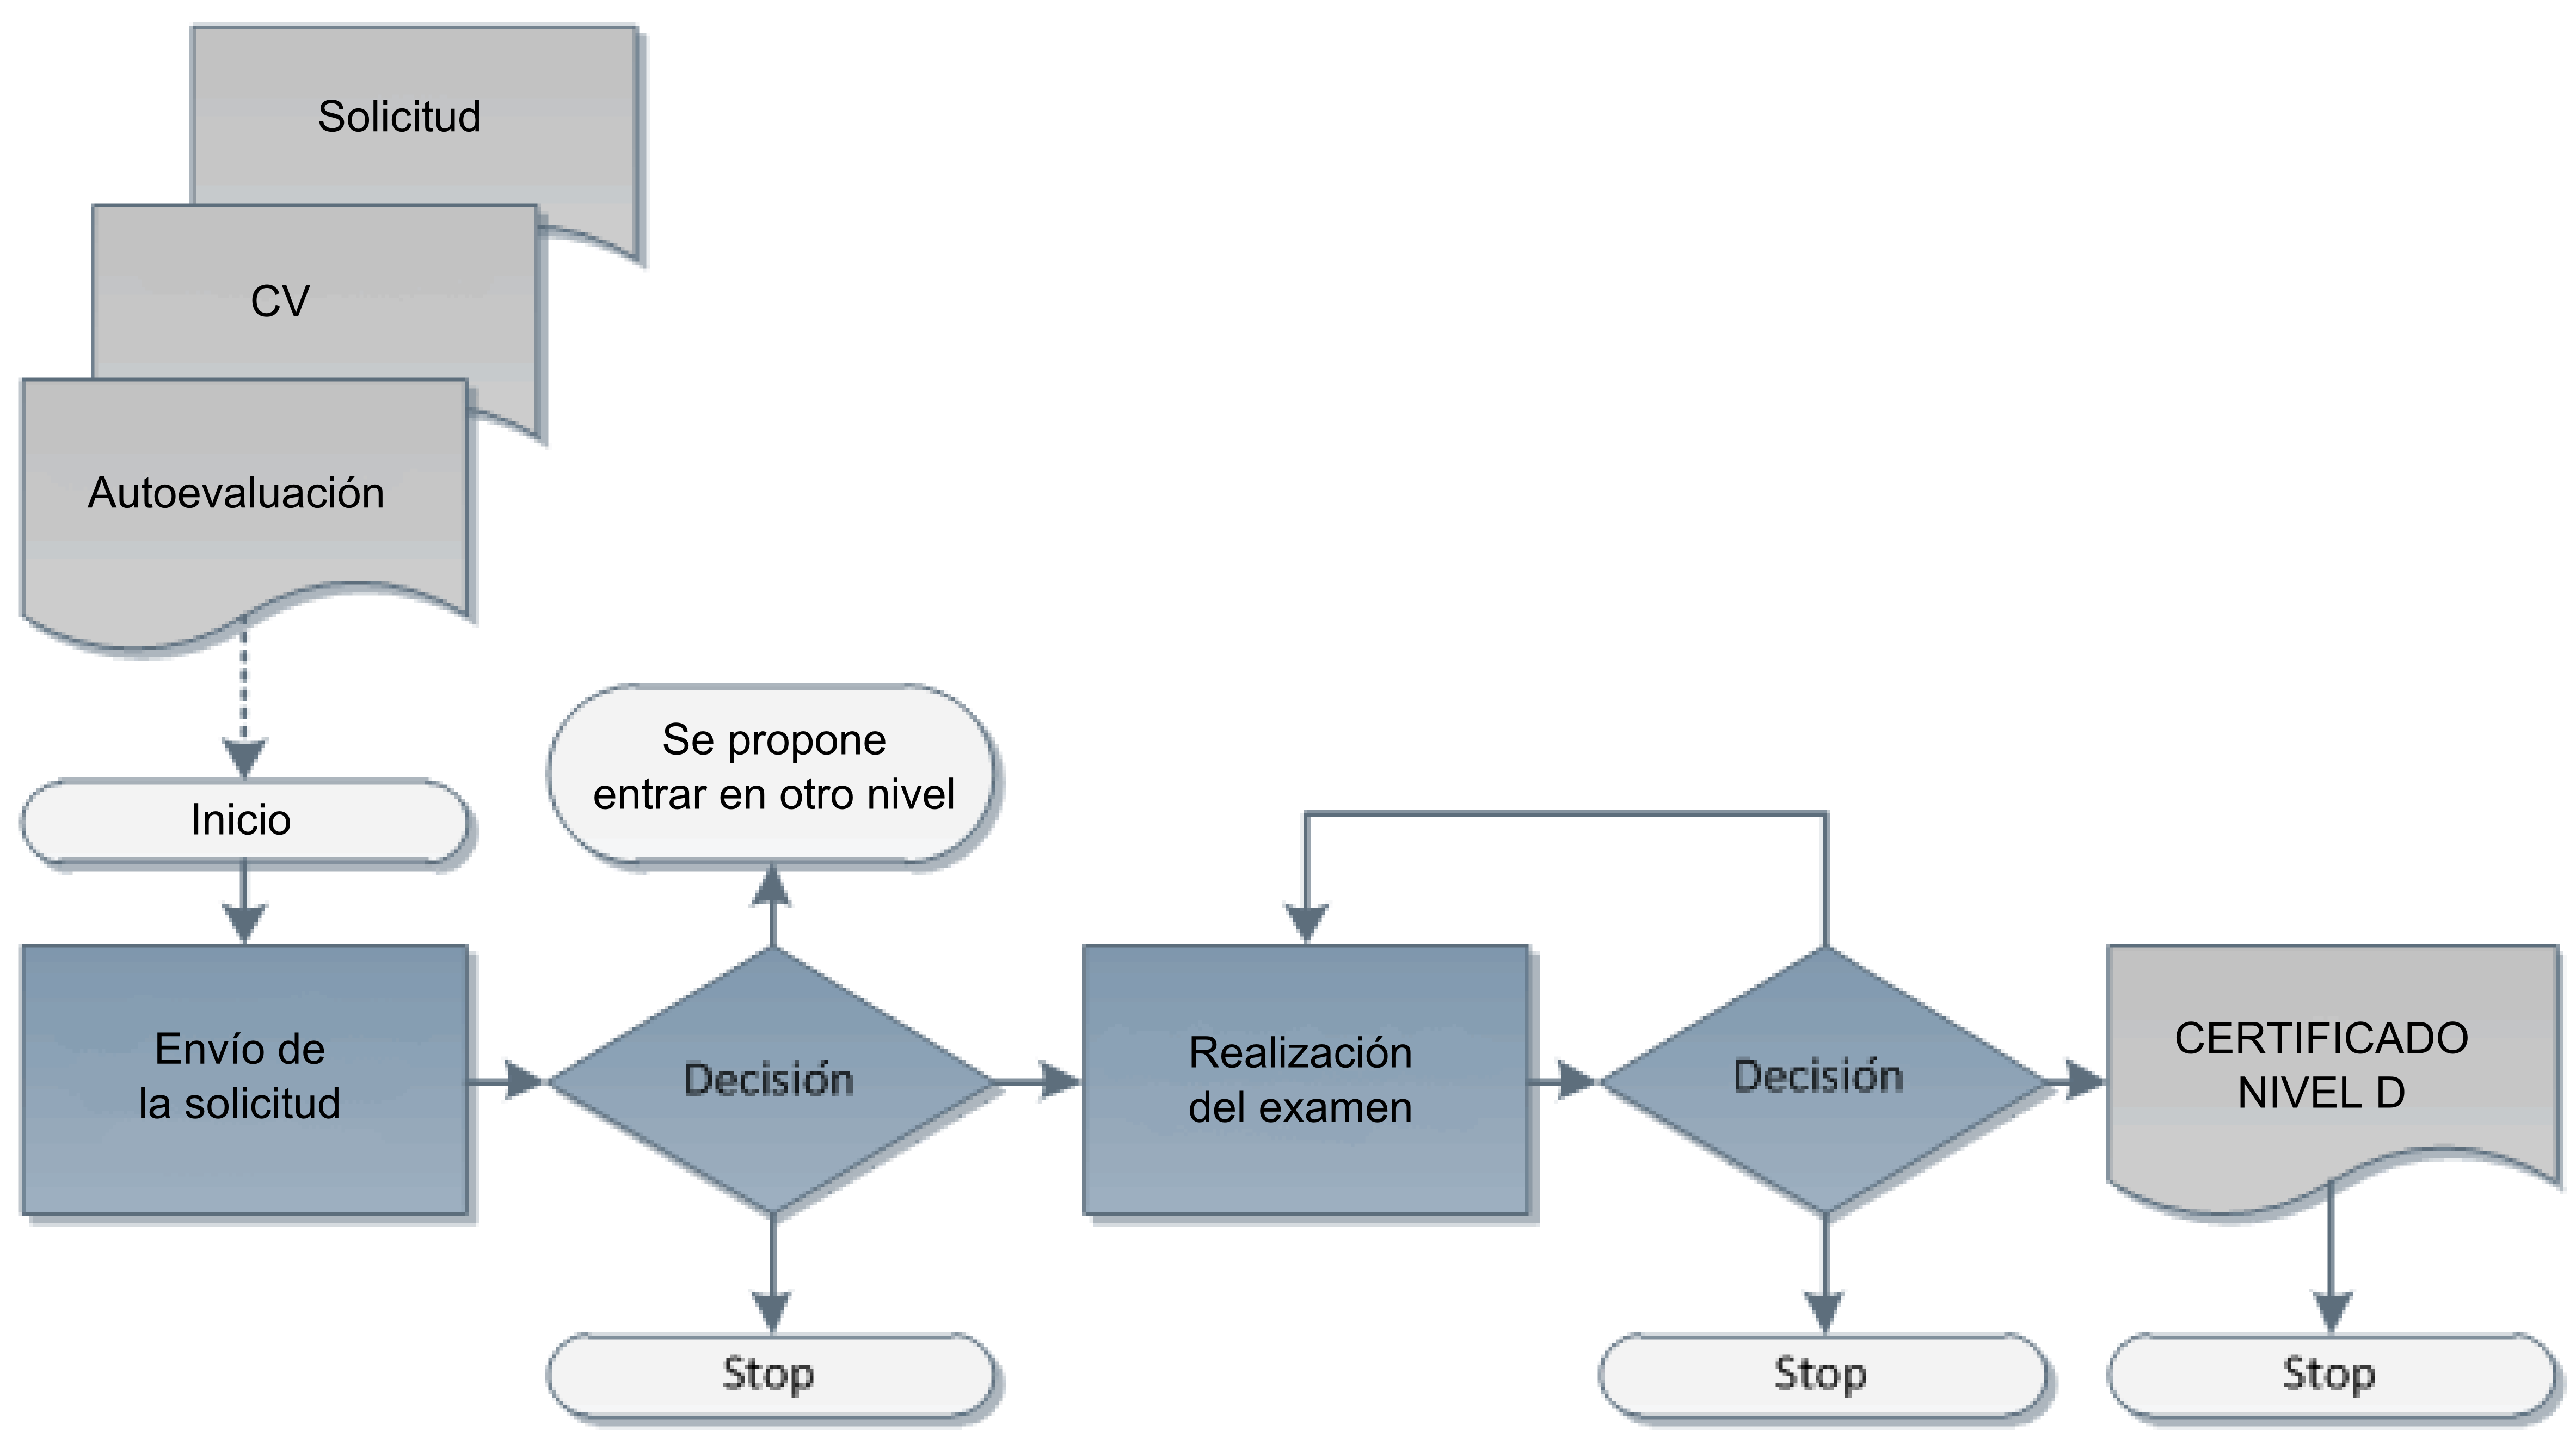
\includegraphics[height=4.5cm]{figuras/procesod.png}
			
			Diagrama de flujo del proceso de certificación.
		\end{center}
		
	\end{enumerate}
	
\end{frame}
